\documentclass{article}

\usepackage[utf8]{inputenc}
\usepackage{graphicx}
\usepackage{float}
\usepackage{makecell}
\usepackage{subcaption}
\usepackage[bottom]{footmisc}

% Enter the name of the subject
\newcommand{\assignmentname}{Game Theory}
% Your names
\newcommand{\studentA}{Meyer Jonathan}
\newcommand{\studentB}{Miroyan Dawid}
\newcommand{\studentC}{Van Herck Caitlin}
\newcommand{\studentD}{Van Wouwe Tom}


\title{\textmd{\textbf{Computationele Biologie}}\\\normalsize\vspace{0.1in}\Large{\assignmentname}\\\vspace{0.1in}\small{\textit{3 Ba INF/WIS/BIO \  2018-2019}}}
\author{\studentA, \studentB, \studentC \ en \studentD}
\date{}

\begin{document}
\maketitle

\section{Inleiding}
De initiële opzet van de informatici in dit project was het bouwen van 'algemene' software die kon gebruikt worden om arbitraire game-theory modellen te simuleren. De idee was om een arbitrair probleem te modelleren a.d.h.v. een \emph{payoff-matrix}, die door de software kon worden ingelezen en gebruikt om de strategieën tegen elkaar af te wegen en de \emph{replicator-formule} kon toepassen om de evolutie van de populaties weer te geven. Vervolgens zouden er ook relevante grafieken kunnen weergegeven worden. De software zou dan getest worden a.d.h.v. bekende gegevens. 
Bij het modelleren werd echter gauw duidelijk dat zulke ‘algemene’ software moeilijk te maken zou zijn, gezien het specifieke biologisch model dat gebruikt werd. Er is dus gekozen voor een meer gespecialiseerd softwaremodel dat eventueel uitbreidbaar is.

\section{Methode}
Het model bestaat uit 2 populaties die met elkaar samenleven. Binnen deze populaties kan men 2 soorten onderscheiden. In geval van ons biologisch model, zijn dit aan de ene kant de \emph{Giver} en \emph{Discriminator} hosts, en aan de andere kant de \emph{mutualist} en \emph{cheater} partners.

\subsection{Config}
De software kan opgedeeld worden in vier aparte onderdelen.
In de configuratie worden de parameters voor de payoffs van de verschillende strategieën. Deze payoffs worden bijgehouden in een matrix, die later doorgegeven wordt aan PayoffMatrix. Doordat er gekozen werd voor een meer gespecialiseerd model, is dit een 2x2 matrix waar je de cellen kan identificeren a.d.h.v. tuples van strategieën. Voor elke populatie moet per strategie gekozen worden hoe groot deze initieel zijn. De som van de groottes is gelijk aan één. Als laatste zijn er simulatie parameters om het aantal iteraties en een stapgrootte te bepalen.
\subsection{PayoffMatrix}
De PayoffMatrix houdt de payoff matrix zelf alsook de verschillende namen van de strategieën bij. Hier zijn ook enkele functies voorzien om het Nash equilibrium en de Evolutionary stable strategies (ESS) te bepalen.

\subsection{Replicator}
De Replicator bevat de logica om de evolutie van populaties te simuleren, deze bevat een methode om de fitness van een soort te bepalen alsook de replicator equation.
De fitness van een strategie $W_m$ wordt gegeven door de volgende vergelijking:
\[ W_m = D \times E(m, D) + G \times E(m, G)\]
met $E(m, D)$ en $E(m, G)$ de verwachte payoffs voor de strategie $W_m$ die associeert met strategieën uit de andere populatie.
De replicator maakt gebruik van
\[\frac{dm}{dt} = m \times c \times (W_m - W_c),\]
\[\frac{dD}{dt} = D \times G \times (W_D - W_G),\]
om de verandering in grootte voor de populaties te bepalen.

\subsection{Graphs}
Hier kunnen enkele grafieken gegenereerd worden. Deze vergelijken de fitness van mutualist partners met cheater partners en discriminator hosts met giver hosts. Er wordt gekenen naar verschillende levels van de discrimination parameters, verschillende groottes van de populatie van mutualist partners en discriminator hosts.

\begin{figure}[h!]
	\centering
	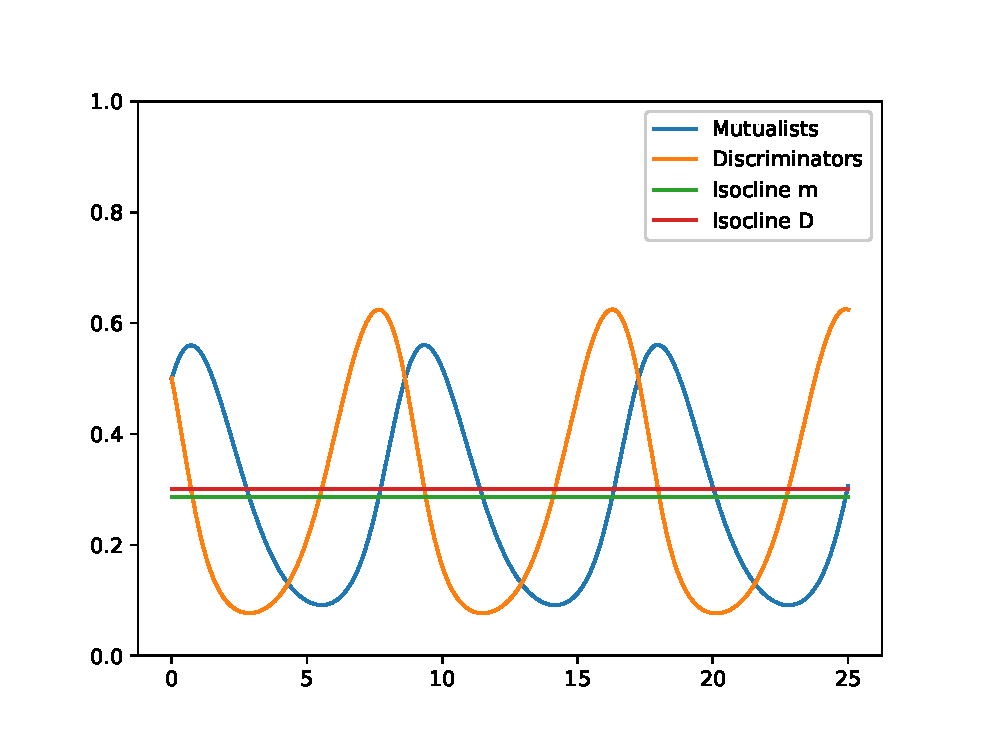
\includegraphics[width=\linewidth]{plots/pop_dynamic.eps}
	\caption{Discriminator hosts D en mutualist partners m over de tijd}
	\label{pop)dynamic}
\end{figure}
\end{document}
